%This document demonstrates proper use of REV\TeX~4 (and
%\LaTeXe) in mansucripts prepared for submission to APS
%journals. Further information can be found in the REV\TeX~4
%documentation included in the distribution or available at
%\url{http://publish.aps.org/revtex4/}. 
% TeX'ing this file requires that you have AMS-LaTeX 2.0 installed
% as well as the rest of the prerequisites for REVTeX 4.0 .
% If you compile your tex files on the Physics
% server, everything is already set up for you.
%

% Choose the format that suits your purposes.  The top line gives the
% two column (twocolumn) format that one sees in printed journals.  The
% second line refers to a one column double spaced format (preprint) that
% is useful during editing.  Use the "%" symbol to edit out the line
% you do not want to use.

\documentclass[twocolumn,preprintnumbers,amsmath,amssymb]{revtex4}
%\documentclass[preprint,showpacs,preprintnumbers,amsmath,amssymb]{revtex4}

% Additional packages needed for graphics, alignment and math fonts.

\usepackage{graphicx}% Include figure files in eps format.
\usepackage{dcolumn}% Align table columns on decimal point.
\usepackage{bm}% bold math.
\usepackage{fixltx2e}
\usepackage{amsmath}
\usepackage{siunitx}
\usepackage{titlesec}
\titlespacing*{\section}{0pt}{1.1\baselineskip}{\baselineskip}


% The \begin{document} command set the start of the RevTeX commands.

\begin{document}

\title{Measurement of the $2^+_2 \rightarrow 2^+_1$ Electric Monopole Transition Strength in $^{110}$Pd for the Study of Nuclear Structure}

\author{Jonah Berean-Dutcher}
\email{jonahberean@alumni.ubc.ca}
\affiliation{Department of Physics and Astronomy, University of British Columbia \\
             6224 Agricultural Road, Vancouver, British Columbia, Canada, V6T 1Z1}

\date{\today}

\begin{abstract}

% A measurement of the strength of the $E0$ transition between the $2^+_2$ and $2^+_1$ nuclear states, of the $^{110}\mathrm{Pd}$ nucleus, is proposed. Analysis will be undertaken of spectroscopic gamma-ray and internal conversion electron data obtained by inelastic scattering of an accelerated alpha particle beam off of a $^{110}\mathrm{Pd}$ target. The multipolarity of nuclear de-excitation between the states of nuclei populated in the study will be determined by studying angular distributions of the associated gamma rays detected in TIGRESS (TRIUMF-ISAC Gamma-Ray Escape Suppressed Spectrometer). The internal conversion coefficient for the transition will be extracted by the combination of TIGRESS data and internal conversion electron emission data collected by SPICE (SPectrometer for Internal Conversion Electrons). \newline 

A measurement of the strength of the $E0$ transition between the $2^+_2$ and $2^+_1$ states, of the nucleus $^{110}\mathrm{Pd}$ is proposed. Analysis will be undertaken of spectroscopic gamma-ray and internal conversion electron data obtained by inelastic scattering of an accelerated alpha particle beam off of a $^{110}\mathrm{Pd}$ target. The $E2/M1$ mixing ratio will be determined from $\gamma$ ray data collected using TIGRESS. The internal conversion coefficient for the transition will be extracted from the combination of TIGRESS data and internal conversion electron data collected by SPICE. These new data will be combined with literature half life and branching ratio information to determine the E0 transition strength for the first time.

\end{abstract}

\maketitle

%%%%% CHECKS (carry over to future docs) %%%%%

% citations. REMOVE EVITTS ORIGINAL, a Krane there.
% references, figures, equations are ordered
% \rho^2 instead of \rho is common error; do search
% references appear before punctuation
% references to nuclei use 'the' not 'a' ... nucleus. 
% use of ` and ' is correct
% mistakes in equations due to copy pasting similar equations and failing to make small changes. seems to be a tendency
% check equation referencing

% LAST: Grammar, Missing Word read through 

%%%%% CHECKS (carry over to future docs) %%%%%

\section{Motivation}

%

The strength of electric monopole ($E0$) transitions in nuclei can provide insight into their nuclear structure. These transitions are particularly sensitive to shape coexistence in nuclei \cite{evitts_1}. $E0$ transitions are a less studied multipolarity of transition, due primarily to the added complexity in performing electron spectroscopy measurements.

This project proposes the study of such a transition in the nucleus $^{110}\mathrm{Pd}$. The determination of the relative probabilities, or strengths of these transition mechanisms provides a key method of studying nuclear structure and behaviour. The measurement of this $E0$ transition strength, $\rho^2(E0)$, would provide a stringent test of the efficacy of nuclear models in describing the nucleus $^{110}\mathrm{Pd}$. 

Despite these implications, the $E0$ transitions are less studied, particularly in comparison to $E2$ transitions. This is reflected in Figure \ref{comparison}, which compares the published literature $E2$ transition strengths, $B(E2)$, (where known) for the $2^+_1 \rightarrow 0^+_1$ transition \cite{evitts_17} against the reported $\rho^2(E0)$ values in the $2^+_2 \rightarrow 2^+_1$ transitions \cite{evitts_5}.  The known $\rho^2(E0)$ are from a 2005 review, however there have been only a small number of additional measurements since this most recent review. Here, the numeric subscript is used to denote specifically the decay of the lowest-lying excitation of the given spin to the ground state of the nucleus. The $B(E2)$ values are given in Weisskopf units (W.u.), which are based on single particle estimates of the transition. The dimensions of these units are dependent upon the transition multipolarity, and as such are not `universal' in the usual sense of a physical unit \cite{evitts_4}. The $\rho^2(E0)$ values are dimensionless but are usually on the order of $10^{-3}$, so they are displayed in milliunits. The grey dashed lines show the closed nuclear shells, and in the upper plot these correspond clearly to lower $B(E2)$ values. The $B(E2)$ values are seen to increase when moving towards the mid-shell regions. Distinct trends cannot be discerned in the lower plot, due to lack of measured values. This insufficiency underscores the motivation for further $\rho^2(E0)$ measurements to be made.
\begin{figure}[!hht]
  \centering
  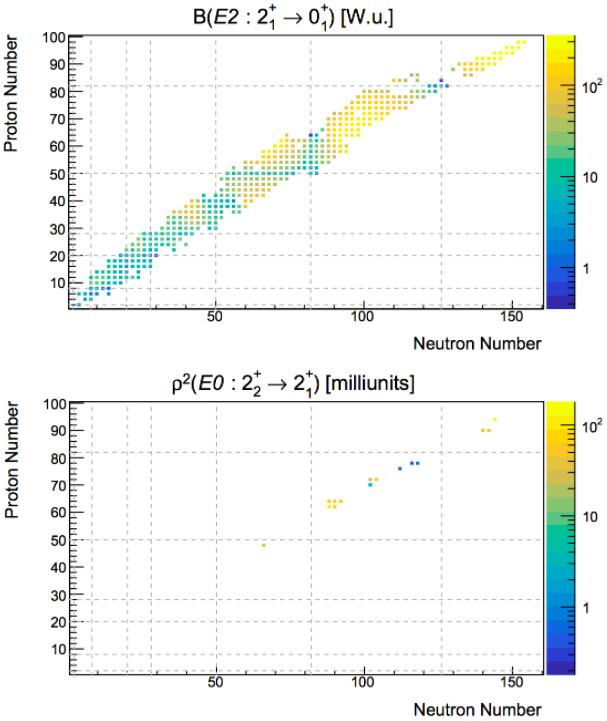
\includegraphics[width=0.45\textwidth, height=0.6\textwidth,keepaspectratio]{EvittsE2E0.png}
  \caption{A comparison between (top) the known $B(E2)$ values between the first $2^+$ and ground state (2016) \cite{evitts_17}, and (bottom) the known $\rho^2(E0)$ values for the second excited $2^+$ to the first excited $2^+$ state (2005) \cite{evitts_5} of even-even nuclei. Image from Ref \cite{EVITTS}.}
  \label{comparison}
\end{figure}

A measurement of $\rho^2(E0)$ in this nucleus would provide a valuable benchmark for application in models of nuclear shape and collective excitations. For nuclei in the mid-shell region, models that focus on the collective nature of the nucleus may be used \cite{evitts_4}. Macroscopic behaviors, such as vibrations of spherical nuclei and axially symmetric rotations of deformed nuclei, are considered in an alternative approach to the idealized approach of the spherical shell model. $^{110}\mathrm{Pd}$ lies in such a mid-shell region, thus making it an important constituent in the broader study of nuclear structure physics. 

\section{Theory}

\subsection{Collective Models of Nuclear Structure}

The shell model of the nucleus is an approximation that often fails to properly describe nuclei in the region away from closed shells. In these regions, the large number of valence nucleons interact in such a way that leads to deviations away from a deformed nuclear potential \cite{evitts_74}. For these regions an alternative model may be used that focuses on the collective nature of the nucleus. In non-spherical nuclei the deformation parameter, $\beta$ may be related to the eccentricity of the ellipsoid by
\begin{gather}
\beta = \frac{4}{3}\sqrt{\frac{\pi}{5}}\frac{\Delta R}{R_{\mathrm{AVG}}}
\label{beta}
\end{gather}
where $\Delta R$ is the difference between the semi-major and semi-minor axes of the ellipsoid and $R_{AVG}=1.3A^{1/3} \si{fm}$, with $A$ being the atomic mass number. When $\beta>0$ the nucleus is prolate, and when $\beta<0$ the nucleus is oblate \cite{evitts_4}. The excitation energies of an idealized deformed, axially-symmetric rotating nucleus are given be
\begin{gather}
E = \frac{\hbar^2}{2I}J(J+1)
\label{rotationalEnergies}
\end{gather}
where $I$ is the moment of inertia. The addition of rotational energy results in higher excited states with larger spin. Equation (\ref{rotationalEnergies}) is used to determine the idealized excitation energies of higher lying states; for example, in a nucleus of even number of protons and even number of neutrons the ground state is $0^+$ and the energies are
\begin{equation}
\begin{aligned}
E(0^+) ={} & 0 \\
E(2^+) ={} & 6(\hbar/2I) \\
E(4^+) ={} & 20(\hbar/2I)
\label{Energies}
\end{aligned}
\end{equation}
Thus, the ratio of $4^+_1/2^+_1$ energies in a rigidly-deformed rotational nucleus is 3.33. Only even values of $J$ are considered due to the coupling of an even number of spins within the nucleus \cite{evitts_4}. Generally, the ratio of $4^+_1/2^+_1$ energies is an indication of the macroscopic behaviour of the nucleus. In the regions between closed shells, this ratio ranges from 3.33 in rotational nuclei to 2.0 for nuclei that behave as spherical vibrators. Nuclei with intermediate values are described as the transitional nuclei between these two cases.

In Figure \ref{levels} the energy levels of the first two intrinsic excitations are shown for the nucleus $^{110}\mathrm{Pd}$. The ratio of $4^+_1/2^+_1$ is {\raise.17ex\hbox{$\scriptstyle\sim$}}2.46, indicating a transitional structure for this nucleus. 
\begin{figure}[!ht]
  \centering
  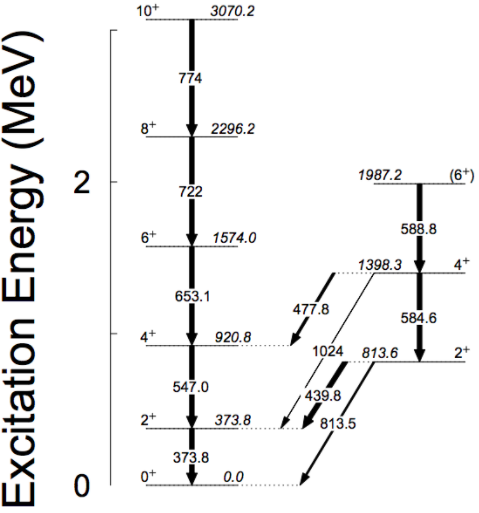
\includegraphics[width=0.5\textwidth,height=0.36\textwidth,keepaspectratio]{Levels.PNG}
  \caption{Energy levels in the first two intrinsic excitations for the nucleus $^{110}\mathrm{Pd}$. State and transition energies are given in keV. The spin and parity of each state is labeled. Image from Ref\cite{NNDC}.}
  \label{levels}
\end{figure} 
States of the same spin and parity (with similar excitation energies) but different intrinsic shapes can mix such that the resultant state is an admixture of shapes. Additionally, processes exist that can create low-energy states with different deformations to the ground state, leading to the phenomena of shape coexistence.

\subsection{Nuclear Transitions and Multipolarities}

When excited nuclear states decay, they do so through transitions involving energy emission. The energy emitted from the nucleus may be in the form of photons, or particles. The dominant way that this occurs is through the emission of $\gamma$ rays. An emitted $\gamma$ ray will carry away energy equal to the difference in energy between the initial and final states of the transition. The emitted gamma rays can be characterized by the electromagnetic multipolarity of the associated transition. These multipolarities define the angular momentum, parity and angular distribution of the gamma ray emission in space. The angular momentum of the nuclear transition, and subsequently the $\gamma$ ray emitted, is governed by a set of selection rules, in conjunction with the parity \cite{EVITTS}.

If the spin and parity of the two nuclear energy levels is given by $J^{\pi_i}_{i}$ and $J^{\pi_f}_{f}$, then the angular momentum carried away by the $\gamma$ ray, $L$, can take values in the following range
\begin{equation}
|J_i-J_f|\leq L \leq J_i+J_f
\end{equation}
Additionally, $\gamma$ rays must carry away at least 1 $\hbar$ unit of angular momentum, thus forbidding gamma ray emission as a mechanism for transitions between two nuclear states of spin 0. Transitions of this nature must occur by other mechanisms, such as internal conversion electrons or internal pair formation \cite{evitts_4}. 
Electromagnetic multipole fields are classified as either electric or magnetic in nature according to specific parity rules. If an electric transition has even $L$ then there is no change in parity but if $L$ is odd then there is a change of parity. The inverse rule defines magnetic transitions. i.e.
\begin{equation}
\begin{aligned}
&\pi(EL)=(-1)^{L} \\
&\pi(ML)=(-1)^{L+1}
\label{selectionRules}
\end{aligned}
\end{equation}
Combined, these selection rules define the allowed multipolarities for a given transition. For example, in a $2^+$ to $2^+$ transition, the $M1$, $E2$, $M3$ and $E4$ processes will all have non-zero probability. There is also the $E0$ transition available but this will not decay through the emission of a $\gamma$ ray and will instead decay through alternate methods such as internal conversion \cite{evitts_4}. 

\subsection{Gamma-Ray Angular Correlations}
For the mixed $2^+ \rightarrow 2^+$ transition, it is necessary to determine the relative intensities of the possible multipolarities of $\gamma$ ray decay. The transition from one state to another can be thought of as an electromagnetic multipole operator, acting on an initial nuclear wavefunction to transform it into a final wavefunction. The transition between two given states is defined by the matrix element of this multipole operator \cite{evitts_4}. The mixing ratio, $\delta$, is defined as the fraction of $E2$ to $M1$ matrix elements.

The angular distribution of $\gamma$ rays can be described by \cite{evitts_83}
\begin{gather}
W(\theta) = N\cdot[1+a_2P_2(\cos \theta) + a_4P_4(\cos \theta)]
\label{angularDistro}
\end{gather} 
where $N$ is a normalization parameter, $P_\eta(\cos \theta)$ are the Legendre Polynomials
\begin{equation}
\begin{aligned}
P_2(\cos \theta) ={}& \frac{1}{2}\cdot (3 \cos^2 \theta - 1) \\
P_4(\cos \theta) ={}& \frac{1}{8}\cdot (35 \cos^4 \theta - 30 \cos^2 \theta + 3)
\label{legendre}
\end{aligned}
\end{equation}
$a_\eta$ are the coefficients which depend on the parent spin and the mixing ratio of the transition. 

% $a_\eta=\alpha_\eta A_\eta$ are coefficients; $\alpha_\eta$ is the attenuation coefficient of the alignment and $A_\eta$ is the angular distribution coefficient. $A_\eta$ is dependent on the spins of the initial and final states, the multipolarity of the transition, and the mixing ratio. These calculated coefficients are tabulated by Yamazaki \cite{evitts_83}.

% $\alpha_\eta$ describes the population distribution of the magnetic substates of the initial state. The alignment of a state is lower if there is a greater population of the $m =0$ substate. If there is only one magnetic substate, then the total angular distribution of $\gamma$ rays will be isotropic. 

\subsection{Internal Conversion Decay and $\rho^2(E0)$}

$E0$ transitions cannot occur by $\gamma$ ray emission due to the requirement for the photon to carry at least one unit of angular momentum. These transitions must occur by alternate modes, such as the emission of two photons ($\gamma \gamma$), production of an electron-positron pair (internal pair formation, $\pi$), or internal conversion electron decay.
In internal conversion electron decay, the energy is released via the emission of one of the orbital electrons, with energy equal to the transition energy less the binding energy of the particular atomic orbital, $B_e$, i.e.
\begin{gather}
T_e = T_\gamma - B_e
\label{iceEnergy}
\end{gather}
% In an energy spectrum corresponding to internal conversion electron decay, separate peaks would be observed for the different electron shells. Electrons in the different shells have different binding energies, resulting in different emitted electron energies according to (\ref{iceEnergy}). The most dominant peak will be from the K shell electrons, orbiting closest to the nucleus, and subsequently possessing the greatest spatial overlap of electron and nuclear wave functions. 
The total decay probability of a nuclear transition is equal to the sum of probabilities for the individual decay modes i.e.
\begin{gather}
\lambda_t = \lambda_\gamma + \lambda_e + \lambda_{\gamma \gamma} + \lambda_\pi +...
\label{totalDecay}
\end{gather}
This can be rearranged as
\begin{gather}
\lambda_t = \lambda_\gamma(1+\alpha_e+\alpha_{\gamma \gamma}+ \alpha_\pi+...)
\label{iceCoeff}
\end{gather}
where $\alpha_x=\lambda_x/\lambda_\gamma$ is the coefficient of the specific decay mode, defined as a probability of that mode relative to $\gamma$ ray decay. $\alpha_e$ is the internal conversion coefficient \cite{evitts_4}.

The $E2/M1$ mixing ratio and the internal conversion coefficient are both required for the calculation of $q^2$, which is the ratio of intensities between $E0$ and $E2$ transitions from a common initial state. Given by $q^2 = I(E0)/I(E2)$. For a $2^+\rightarrow2^+$ transition, the mixing of $E0$, $M1$ and $E2$ components (higher $L$ components may be neglected) results in a $q^2$ determined by
\begin{gather}
q^2 = \frac{\alpha_\mathrm{exp}(1+\delta^2)-\alpha(M1)}{\alpha(E2)\cdot \delta^2}-1
\label{qSquared}
\end{gather}
where $\alpha$ are theoretical conversion coefficients obtained from BrIcc \cite{evitts_86_BrIcc}, and $\alpha_\mathrm{exp}$ is an experimentally determined value of the internal conversion coefficient (i.e. ratio of $E0+M1+E2$ electrons vs. $M1+E2$ $\gamma$ rays). Using these experimental inputs, $\rho^2(E0)$ may be calculated from

\begin{gather}
\rho^2(E0) = q^2 \times \frac{\alpha(E2)}{\Omega(E0)} \times W_\gamma(E2)
\label{E0Strength}
\end{gather}
where $\Omega(E0)$ is an electronic factor from atomic theory and $W_\gamma(E2)$ is the $E2$ transition rate, a previously measured value available from NNDC \cite{NNDC}.

\section{Details on Proposed Experiment/Calculation} 
The proposed study will investigate data obtained by inelastic scattering of an accelerated alpha particle beam off of a $^{110}\mathrm{Pd}$ target. The incident alpha particle beam interacted with the target at an energy above the Coulomb barrier; the energy barrier due to electrostatic interaction that two nuclei must surpass in order to undergo a nuclear reaction. This $^{110}\mathrm{Pd}$ experiment utilized SPICE (SPectrometer for Internal Conversion Electrons) for detection of internal conversion electrons, and the TIGRESS (TRIUMF-ISAC Gamma-Ray Escape Suppressed Spectrometer) high-purity germanium array for detection of emitted $\gamma$ rays. SPICE was equipped with an S3 type silicon CD detector for the detection of coincident alpha-particle recoils downstream of the target. A schematic diagram of the experiment is shown in Figure \ref{diagram}. A 35.6 MeV beam of alpha particles was sent down the beamline at TRIUMF's Isotope Separator and Accelerator (ISAC-II) onto a $^{110}\mathrm{Pd}$ target \cite{SPICE,TIGRESS}. 
\begin{figure}[!ht]
  \centering
  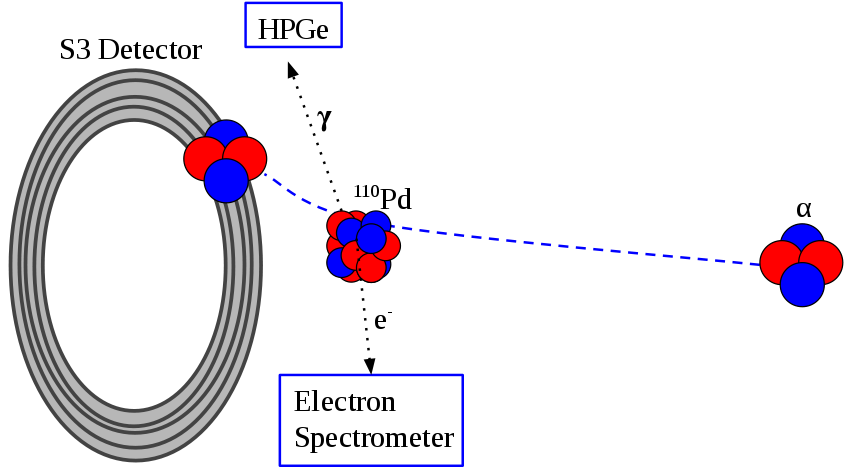
\includegraphics[width=0.45\textwidth,keepaspectratio]{ExperimentSchematic.png}
  \caption{Diagram showing the setup for the experiment, with an alpha nucleus scattering off a $^{110}\mathrm{Pd}$ target nucleus into the S3 detector; emitting electrons and $\gamma$ rays.}
  \label{diagram}
\end{figure}

% From the $\gamma$ ray spectra collected by TIGRESS, the ($E2/M1$) mixing ratio is to be determined via analysis of angular distributions. For the transition of interest, $2^+_2 \rightarrow 2^+_1$, the attenuation coefficient of the alignment can be determined by fitting Equation (\ref{angularDistro}) to the distribution from the initial $2^+$ state to the $0^+$ ground state. Since this transition is a pure $E2$ transition, the multipolarity is known exactly, and there is no mixing ratio to consider. The tabulated angular distribution coefficients can be fixed, and the alignment coefficient extracted from the fit. 

% With $\a_\eta$ fitted, the mixing ratio can be determined analogously, by holding $\alpha_\eta$ and $A_\eta$ constant for a fit to determine $\delta$.

From the $\gamma$ ray spectra collected by TIGRESS, the ($E2/M1$) mixing ratio is to be determined via analysis of angular distributions. For the transition of interest, $2^+_2 \rightarrow 2^+_1$, the coefficients $a_\eta$ can be determined by normalizing Equation (\ref{angularDistro}) to the distribution from the initial $2^+$ state to the $0^+$ ground state. Since this transition is a pure $E2$ transition, the multipolarity is known exactly, and there is no mixing ratio to consider. The mixing ratio can then be extracted from study of the angular distribution from the transition of interest.

The internal conversion coefficient is to be obtained by a comparison of the $e^-$ and $\gamma$ ray spectra. This is achieved via the ratio of measured counts, $A$, multiplied by the absolute efficiencies, $\epsilon$, i.e.
\begin{gather}
\alpha = \frac{A_e}{A_\gamma} \cdot \frac{\epsilon_\gamma}{\epsilon_e}
\label{findICE}
\end{gather}
Finally using Equation (\ref{E0Strength}), the $\rho^2(E0)$ can be calculated. 

\section{Resources List}
The project will require the computing resources of the Gamma-Ray Spectroscopy Group at TRIUMF's ISAC facility. A workspace and computer have been provided. The analysis will use specifically made tools in the ROOT framework, and the GRSISort data sorting package. The calculation of $\rho^2(E0)$ relies on nuclear databases and previously tabulated values such as BrIcc, NNDC, and angular distribution coefficients \cite{evitts_86_BrIcc,evitts_83,NNDC}. 
\vspace{18pt}
\section{Planned Schedule}
The following schedule is for the analysis period of the project. All analysis is expected to be completed by the end of February, thus leaving March for publication and thesis writing. \newline
\underline{December}: The measurement of absolute internal conversion coefficients. This requires a study of the relative efficiency curves between the SPICE and TIGRESS detectors. These efficiencies will be scaled to fit the data, before proceeding with a determination of efficiency of the data acquisition system. Known internal conversion coefficient values will be used for normalization, preceding absolute measurement of the internal conversion coefficient. \newline 
\underline{January}: The measurement of $\delta(E2/M1)$. Data will be resorted into the required format for angular distribution analysis. Using pure $E2$ transitions, as described above, the measurement technique will be normalized over a range of known transitions. Analysis of the angular distribution of the transition of interest will yield a measurement of $\delta(E2/M1)$. \newline
\underline{February}: Calculation of $\rho^2(E0)$. A full error analysis and simulations or calculations from nuclear theory may be required. Analysis will conclude with an interpretation of the results in the context of known physics. 

\begin{thebibliography}{99}

\bibitem{evitts_1} J.L. Wood et al. Electric monopole transitions from low energy excitations. \textit{Nuclear Physics A}, 651:323-368, 1999.
\bibitem{evitts_17} B. Pritychenko et al. Tables of E2 transition probabilities from the yrast states in even-even nuclei. \textit{Atomic Data and Nuclear Data Tables,} 107:1-139, 2016.
\bibitem{evitts_5} T. Kibedi and R.H. Spear. Electric monopole transitions between 0+ states. \textit{Atomic Data and Nuclear Data Tables,} 89(1):77-100, 2005.
\bibitem{evitts_4} K.S. Krane. \textit{Introductory Nuclear Physics.} John Wiley and Sons, 1988.
\bibitem{EVITTS} L. J. Evitts. Ph.D. thesis, University of Surrey, 2017.
\bibitem{evitts_74} R.F. Casten. \textit{Nuclear Structure from a Simple Perspective.} Oxford University Press, 1990.
\bibitem{NNDC} S.Lalkovski et al. Two-quasiparticle and collective excitations in transitional $^{108,110}\mathrm{Pd}$ nuclei. \textit{Eur.Phys.J. A} 18, 589 (2003)
\bibitem{evitts_83} T Yamazaki. Tables of coefficients for angular distribution of gamma rays from aligned nuclei. \textit{Nuclear Data Sheets. Section A,} 3(1):1-23, 1967.
\bibitem{evitts_86_BrIcc} T. Kib\'edi et al. Evaluation of theoretical conversion coefficients using BrIcc. \textit{Nuclear Instruments and Methods A} 589(2):202-229, 2008.
\bibitem{TIGRESS} G. Hackman and C. E. Svensson. The triumf-isac gamma-ray escape suppressed spectrometer, tigress. \textit{Hyperfine Interactions,} 225(1):241–251, Jan 2014.
\bibitem{SPICE} J. Smallcombe et al. SPectrometer for Internal Conversion Electrons (SPICE) at TRIUMF-ISAC. 	
\textit{EPJ Web Conf.} 123 (2016) 04005, Sep 2016.

\end{thebibliography}

\end{document}
%
% ****** End of file  ******